\chapter{延迟强化学习}
\label{chap:delay}

\section{引言}
\label{sec:delay_intro}

尽管\glspl{mdp}具有通用性，但仍无法把握许多序列决策问题的复杂性。例如，\gls{pomdp}便是如此。
本章旨在扩展原始框架，引入延迟（delay）概念。
延迟可能出现在状态观测、动作执行或奖励收集中。
状态观测延迟（state observation delay）指智能体观测到的状态并非环境当前状态，而是过去某一时刻的状态。
但智能体仍须选择一个将施加于当前未观测状态的动作。
在动作执行延迟（action execution delay）情形下\footnote{此处沿用\cite{derman2021acting}的命名法。}，智能体所选择的动作将施加于未来某一状态。
相反，施加于当前状态的动作是智能体在过去选择的。
如上文所述，前两类延迟相似，而最后一种延迟——奖励收集延迟（reward collection delay）——则略有不同。
奖励收集延迟指智能体在转换发生后若干步才获得该转换对应的奖励。
将奖励分配至正确转换时，考虑此类延迟尤为重要。
因此，这类延迟可能涉及信用分配（credit assignment）问题，主要在在线学习方法中研究，在奖励收集过程中高效学习至关重要。

延迟在\gls{rl}应用中普遍存在，但通常未被考虑，从而导致次优行为。
值得注意的是，在仿真中训练并针对现实问题测试是延迟可能产生危害的典型场景。
在仿真中忽略物理传感器或执行器引入的延迟十分常见。
然而，这些延迟可能是从仿真迁移到现实时性能下降的根源。

本章首先提出统一\gls{rl}中延迟问题的符号表示。
我们定义了延迟\glspl{mdp}，即在\gls{mdp}框架基础上引入延迟的序列决策过程扩展。
然后，介绍文献和实践中遇到的主要延迟类型。
最后，讨论延迟\gls{rl}及相关领域的文献。
现有文献综述尚不完善，且先前工作中结果重叠现象普遍存在。

\section{符号表示}
\label{subsec:delay_notation}

下面给出延迟\gls{mdp}的通用定义，将文献中遇到的大多数延迟类型作为特例包含在内。
记\gls{dmdp}为延迟\gls{mdp}\footnote{记号DMDP可能更直观，但该缩写已在文献中广泛用于指代确定性\glspl{mdp}或折扣\glspl{mdp}。
该缩写也由本文所用的延迟记号所佐证。}。
\gls{dmdp}源于一个\gls{mdp}并附有三组序列变量：动作执行延迟$(\delay_t^a)_{t\in\naturalnumbers}$；状态观测延迟$(\delay_t^s)_{t\in\naturalnumbers}$；奖励收集延迟$(\delay_t^r)_{t\in\naturalnumbers}$。
注意这一记号突出了延迟可能随时间变化。
在文献中，延迟通常被假设为马尔可夫过程，即$\delay_t \sim P(\cdot\vert \delay_{t-1}, s_{t-1}, a_{t-1})$。
该定义包括$\delay_t \sim P(\cdot\vert s_{t-1})$时的状态相关延迟、$\delay_t \sim P(\cdot\vert\delay_{t-1})$时的马尔可夫链延迟以及$(\delay_t)_{t\in\naturalnumbers}$为独立同分布时的随机延迟。

\section{延迟的性质}
\label{sec:nature_delays}

从\gls{dmdp}的通用定义出发，可以研究许多子情形。
本节旨在给出文献或实际\gls{rl}应用中遇到的延迟类型概览。首先介绍定义延迟的不同属性。
最后给出本论文关于延迟的假设。

\begin{figure}[t]
    \centering
    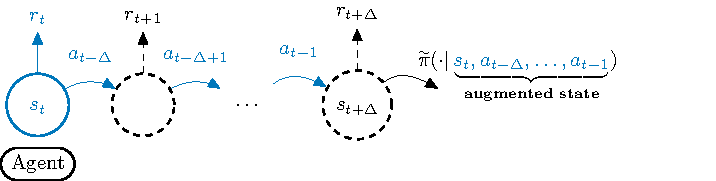
\includegraphics[bylabel=undelayedmdp]{img/thesis_plots.pdf}
    \caption{无延迟\gls{mdp}的表示。}
    \label{fig:undelayed_mdp}
\end{figure}

\subsection{常值延迟与随机延迟}
\label{subsec:constant_stoch_delays}
如前所述，延迟是随机变量，但文献中通常假设常值延迟（constant delay）。
这一简化模型对许多应用而言已足够现实，尤其是当延迟的潜在随机性相对于过程步长可忽略不计时。
例如，\cite{ramstedt2019real}在自动驾驶仿真和连续机器人运动控制中考虑1步常值延迟；\cite{hester2013texplore}在自动驾驶中考虑2步延迟；\cite{walsh2009learning}在简单仿真任务（包括网格世界）中考虑1到20之间的各种延迟。
在主动流动控制中，延迟甚至可达63步\cite{mao2022active}。
然而，对于某些应用，必须对延迟的随机性进行建模。
在\cite{bouteiller2020reinforcement}中，随机延迟（stochastic delay）由策略通过WiFi传输至飞行机器人以及观测数据回传所引起。
\cite{campbell2016multiple}研究了泊松分布延迟对Q学习的影响。
总的来说，即使实际延迟通常非常值，假设常值延迟是为了简化问题，前提是延迟的变化对模型性能不关键。

\subsection{状态观测延迟与动作执行延迟}
\label{subsec:state_action_delays}
当智能体无法获知当前状态但能访问\gls{mdp}的历史状态时，即出现状态观测延迟（state observation delay）。
这与\gls{pomdp}形成对比：在\gls{pomdp}中，历史状态通常不向智能体公开，而是揭示关于当前状态的某些部分信息。\Cref{fig:state_obs_delayed_mdp}展示了状态观测延迟的示例，与之对比的是\Cref{fig:undelayed_mdp}中的无延迟\gls{mdp}。
在图示中，读者可能注意到增广状态（augmented state）这一概念，即最后观测到的状态$s_{t-\delay}$与智能体在过去已选择但尚未观测到结果的所有动作$a_{t-\delay},\dots,a_{t-1}$的拼接。
这一概念是延迟强化学习的核心。
实际上，通过考虑增广状态，智能体汇集了关于延迟过程的所有可能信息。
在马尔可夫性质下，考虑比$s_{t-\delay}$和$a_{t-\delay}$更早的状态或动作将是冗余的。

动作执行延迟（action execution delay）发生在智能体虽然观测到当前状态，但选择的动作将在未来若干步之后才执行的情况。
\Cref{fig:action_exec_delayed_mdp}展示了动作执行延迟的示例。
注意此情形下增广状态的定义。
与状态观测延迟类似，增广状态穷尽描述了延迟环境。
另一个有趣之处在于时间索引。
对于动作执行延迟，智能体在时间$t$选择的动作记为$a_t$。
由于延迟，该动作将在时间$t+\delay$施加于状态$s_{t+\delay}$。
这与状态观测延迟形成对比：在状态观测延迟中，智能体在时间$t$选择的动作$a_t$将施加于当前未观测的状态$s_t$。
对于常值延迟，可以将动作索引偏移$\delay$，使得动作$a_t$如无延迟\gls{mdp}那样施加于$s_t$。
但这仅对常值延迟\gls{mdp}可行。
若延迟为随机，则智能体在时间$t$选择的动作标签将是随机的。
此外，若两个动作因随机延迟同时施加，它们将被赋予相同索引。
这似乎不是良好的命名方式。
因此，无论在何种情形下，本文使用智能体选择动作的时间作为该动作的索引。
该记号的另一优势在于，如\Cref{fig:state_obs_delayed_mdp}和\Cref{fig:action_exec_delayed_mdp}所示，状态观测延迟和动作执行延迟的增广状态相同。

\begin{figure}[t]
    \centering
    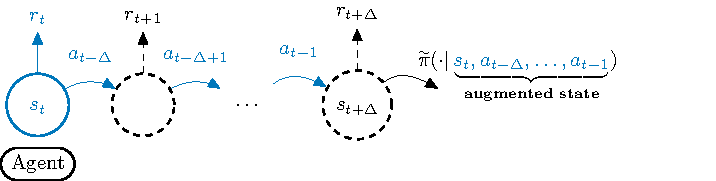
\includegraphics[bylabel=stateobsdelayedmdp]{img/thesis_plots.pdf}
    \caption{具有状态观测延迟的\gls{dmdp}的表示。}
    \label{fig:state_obs_delayed_mdp}
\end{figure}

\begin{figure}[t]
    \centering
    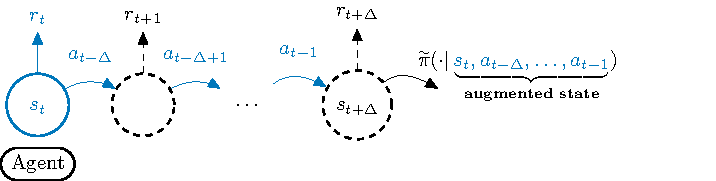
\includegraphics[bylabel=actionexecdelayedmdp]{img/thesis_plots.pdf}
    \caption{具有动作执行延迟的\gls{dmdp}的表示。}
    \label{fig:action_exec_delayed_mdp}
\end{figure}

后文将看到，动作执行延迟和状态观测延迟是等价的，其效应可叠加（\Cref{subsubsec:equiv_action_state_delays}）。
因此，在上图中刻意以类似方式表示这两类延迟。
其增广状态遵循相似构造，且对于相同延迟量包含相同数量的项。
然而，如下文所述，存在一些微小差异，但只要避免混淆就不影响理论分析。
正如\cite{chen2021delay}所指出的，动作执行延迟可能引起一个小问题：延迟可分为两部分——动作选择和动作执行。
前者是智能体在观测到最新状态后计算动作所需的时间。
后者是智能体在环境中实际执行该动作所需的时间。
后者来源是传统意义上的动作执行延迟，而前者来源在实践中可能造成问题。
实际上，若环境在智能体仍在计算前一个动作时提供了新状态（即动作选择延迟长于环境步长），则智能体尚不知晓其前一个动作。
这对之前介绍的增广方法构成问题，我们将在\Cref{sec:related_works}中详细讨论。
这些方法基于先前动作选择当前动作。
因此，此处先前动作集合中缺失了一个动作。
智能体可等待后再计算下一个动作，但延迟将累积，缺失动作的数量会增加。
为避免此类情况，如\cite{chen2021delay}所述，本文假设动作选择延迟小于\gls{mdp}步长\footnote{若实践中不满足此条件，可将动作持续多个步长，以人工创建步长更长的\gls{mdp}，如\cite{metelli2020control}中所述。}。
状态延迟与动作延迟的另一个区别在于奖励收集延迟对二者的影响。
如\cite{katsikopoulos2003markov}所述，在状态观测延迟情形下，若无奖励延迟，智能体观测到与当前未观测状态相关的随机变量的结果。
事实上，当前奖励是当前未观测状态的函数。
换言之，该设置提供了关于当前未观测状态的部分信息。
相反，在动作执行延迟情形下，无奖励延迟不会向智能体提供额外信息，因为最新信息（当前状态）已经是已知的。

\subsection{奖励收集延迟}
\label{subsec:reward_delay}
此处可能需要澄清。
在\gls{rl}文献中，两类不同但相关的问题都可能被称为延迟奖励（delayed reward）。
在许多实际问题中，定义每步奖励可能很困难，而将全部奖励集中到单个步骤中则更容易\cite{han2022off}。
例如，在棋类比赛中为每一步设计奖励很困难，而根据比赛结果给予0或1的奖励则简单得多。
这是第一类延迟奖励，也称为稀疏奖励（sparse reward）。
它通常涉及\gls{mdp}的探索问题。
相反，第二类奖励延迟——奖励收集延迟（reward collection delay）——出现在与转换相关联的奖励（此处定义每步奖励没有问题）在若干步之后才被收集的情况。
后文将看到，这类延迟通常不影响\gls{rl}算法的最终性能，而是影响学习速度。
因此，这两种设定之间的主要区别在于初始奖励的设计方式。
然而，第一种设定可视为第二种设定的特例，即所有奖励均被延迟并在最后一步同时收集。

\subsection{匿名延迟与非匿名延迟}
\label{subsec:anonymous_delays}
可区分匿名延迟（anonymous delay）和非匿名延迟（non-anonymous delay）。
当延迟匿名时，智能体无法获知延迟量；观测状态的时戳可能未向智能体公开。
因此，智能体不再知晓其观测到的所有状态中哪个最新；当前时刻实际执行的动作不明；所收集奖励对应的转换不可知。
因此，匿名性引发信用分配问题。
后文（见\Cref{sec:related_works}）将看到，据我们所知，文献中尚无在\gls{rl}中考虑状态观测或动作执行延迟匿名性的工作。
然而，奖励收集延迟情形下确实考虑了匿名延迟。

\subsection{非整数延迟}
\label{subsec:non_int_delays}
本小节描述延迟如何等于环境步长的非整数倍。
为简化，假设常值延迟。
为清晰起见，假设$\delay\in(0,1)$，但$\delay\in\realnumbers[\ge0]$的一般情形可以类似扩展。
考虑动作执行延迟，但后文将看到状态观测延迟与之等价，可类似定义。

为构建具有非整数延迟（non-integer delay）的过程，可以从连续时间平稳\gls{mdp}出发。
如\cite{sutton1999between}所述，若智能体仅能每隔一个单位时间观测环境，即在时刻$0,1,\dots,t,t+1,\dots$观测，则产生的离散过程是离散时间\gls{mdp}。
记为$\markovdecisionprocess$。
若智能体以相同频率但存在$\delay$的相位偏移进行观测，则时间索引变为$\delay,1+\delay,\dots,t+\delay,t+1+\delay,\dots$。
类似地，这定义了一个离散时间\gls{mdp}，记为$\markovdecisionprocess_\delay$。
由于底层连续时间\gls{mdp}的平稳性，$\markovdecisionprocess$和$\markovdecisionprocess_\delay$具有相同的转移和奖励分布。
下面展示如何利用这两个交错的\gls{mdp}构建$\delay$延迟过程。

由于动作执行延迟，智能体观测到来自$\mathcal{M}$的状态$s_t$，但其动作$a_t$将施加于$\mathcal{M}_\delay$的状态$s_{t+\delay}$，产生奖励$r(s_{t+\delay},a_t)$。
转移概率当然也受影响。
预见到\Cref{subsubsec:theory_augmented_space}的记号，定义$\augmentedbelief(s_{t+\delay}\vert s_t,a)$为在连续时间\gls{mdp}中从$s_t$施加动作$a$经过$\delay$时间单位转移到$s_{t+\delay}$的概率。

由于底层连续时间\gls{mdp}平稳，有$\forall(s,a,s')\in\statespace\times\actionspace\times\statespace$，
\begin{align}
    p(s'\vert s,a)=\int_{\statespace}   \augmentedbelief[1-\delay](s'\vert z,a)\augmentedbelief(z|s,a)\de z.\label{eq:def_p_non_int}
\end{align}
非整数延迟的可视化表示见\Cref{fig:non_int_delay_def}。

\begin{figure}[t]
    \centering
    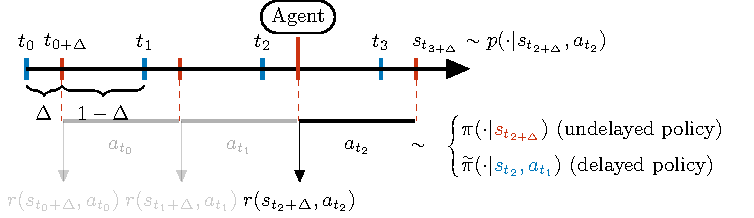
\includegraphics[labelimitation=nonintdelayedmdp]{img/thesis_plots_imitation.pdf}
    \caption{具有非整数动作执行延迟的\gls{dmdp}的表示。}
    \label{fig:non_int_delay_def}
\end{figure}

%=============================================
% 状态相关延迟与动作相关延迟
%---------------------------------------------
\subsection{状态相关延迟与动作相关延迟}
在此设定中，延迟不再独立于智能体的行为。
无论是直接通过动作还是间接通过状态，智能体都可能改变延迟值。
据我们所知，\gls{rl}文献中尚无处理状态相关或动作相关延迟的工作，但实际应用启发这一问题。
例如，使用更复杂的策略选择动作可能获得更优回报，前提是该策略的计算时间合理；当计算时间过大时，使用轻量级策略选择动作则更为合理。
再如，考虑\cite{bouteiller2020reinforcement}中WiFi传输至飞行机器人的设定，延迟很可能取决于机器人与策略计算机之间的距离。

\subsection{关于延迟过程的初始化}
\label{subsec:delay_init}
读者可能会问延迟过程如何初始化。
例如，在状态观测延迟中，如何定义初始状态集合，使得智能体从一开始就有效观测到延迟状态？

这一问题看似浅显，但后文将看到，它可能产生重要的实际影响。
如果仅奖励收集存在延迟，则保持底层\gls{mdp}的初始化方式不会造成问题。
相反，对于动作执行延迟和状态观测延迟，初始化意味着在允许智能体选择任何动作之前，必须以某种方式采样初始的$\delay$个动作。
对于离散或有界动作集，一种任意但合理的采样方案是均匀采样。
这是本文所有实验采用的方法。

注意，取决于初始动作的采样方式以及初始阶段收集的奖励是否计入，智能体的最终回报可能发生显著变化。
举例说明，考虑如下简单\gls{mdp}：奖励等于智能体的速度，且只有一个动作——以固定量"加速"。
在\gls{dmdp}中，初始化意味着"加速"动作在控制权交给智能体之前已经执行了若干次。
这意味着，与初始化速度为0的无延迟智能体相比，延迟智能体在其当前未观测状态中已经累积了速度。
即使初始化阶段的奖励不计入，延迟智能体也以更高的速度起步，从而比无延迟智能体获得更高奖励。
此外，若初始化阶段的奖励计入，则延迟智能体累积更多奖励。
因此，奖励的计入方式可能显著改变延迟智能体相对于无延迟智能体的回报。
我们将这一效应称为延迟初始化偏移（delay initialisation shift）。


\section{相关工作}
\label{sec:related_works}

以下相关工作在各种类型延迟存在时为折扣回报情形提供了理论和实践解决方案，奖励收集延迟除外（\Cref{subsec:reward_delay_related}主要关注平均奖励）。
首先描述文献中解决常值状态观测或动作执行延迟的三种主要方法。
分别是增广状态方法（\Cref{subsec:augmented_related}）、无记忆方法（\Cref{subsec:memoryless}）和基于模型方法（\Cref{subsec:model_based_related_works}）。
然后，将综述范围扩展至更广泛的延迟（仍涉及动作执行和状态观测）；\Cref{subsec:stochastic_related}介绍随机延迟研究，\Cref{subsec:non_int_related}介绍非整数延迟研究。
最后，在\Cref{subsec:reward_delay_related}中讨论奖励收集延迟。

\subsection{常值延迟的增广状态方法}
\label{subsec:augmented_related}

\subsubsection{增广状态的定义}
\label{subsubsec:theory_augmented_space}
本节引入了常值状态观测和动作执行延迟的重要概念。
\cite{bertsekas1987dynamic}和\cite{altman1992closed}分别指出，在动作执行延迟和状态观测延迟情形下，可以通过如下方式增广状态空间将\gls{dmdp}简化为\gls{mdp}。考虑动作执行或状态观测延迟$\delay$；令$(a_1,\dots,a_{\delay})$为智能体已选择但由于延迟尚未观测到结果的最近$\delay$个动作；令$s$为智能体最近观测到的状态。
则增广状态（augmented state）$x=(s,a_1,\dots,a_\delay)$包含该时刻智能体可能收集到的全部信息。
在底层\gls{mdp}的马尔可夫性质下，任何进一步的信息都是冗余的。
\cite{bertsekas1987dynamic,altman1992closed}证明，通过增广状态得到的新过程确实是一个\gls{mdp}。
其新状态空间为$\augmentedstatespace=\statespace\times\actionspace^\delay$。
注意对延迟的指数依赖。
记$\delayedpolicyspace$为依赖于增广状态或增广状态历史的策略集合。
换言之，$\delayedpolicyspace$包含$\policyspace$中任何不依赖比增广状态所含信息更新信息的策略。
增广状态及策略基于增广状态的方式如图\Cref{fig:state_obs_delayed_mdp}和\Cref{fig:action_exec_delayed_mdp}所示。
下面刻画这一过程。对于增广状态$x,x'\in\augmentedstatespace$，满足$x=(s,a_1,\dots,a_{\delay})$和$x'=(s',a_1',\dots,a_{\delay}')$，对于动作$a\in\actionspace$，新的转移函数为\footnote{记号"~~$\widetilde{}$~~"将用于指代延迟量。}
\begin{align*}
    \augmentedtransitionfunction(x'\vert x,a) = p(s'\vert s,a_1)\delta_a(a_{\delay}')\prod_{i=1}^{\delay-1}\delta_{a_{i+1}}(a_{i}'),
\end{align*}
其中Dirac函数的乘积确保动作序列正确地从上一个增广状态传递到下一个。
奖励函数为
\begin{align}
\label{eq:delayed_reward_deterministic}
    \augmentedexpectedrewardfunction(x,a) = r(s,a_1).
\end{align}
如\cite[Lemma~1]{katsikopoulos2003markov}所示，等价形式为
\begin{align}
\label{eq:delayed_reward_expected}
    \augmentedexpectedrewardfunction(x,a) = \expectedvalue_{z\sim \augmentedbelief(\cdot\vert x)} [r(z,a)],
\end{align}
其中$\augmentedbelief$为已知增广状态$x$时当前未知状态$z$的概率。将此概率称为信念（belief），因其与\gls{pomdp}文献中的信念概念相似。
直观上，由于给定动作序列和最近观测状态就能完全确定当前未观测状态的分布，第一个过程在延迟$\delay$步后最终将与第二个过程在期望意义下收集相同奖励。
因此，两个过程中的最优策略对应。
但注意，由于\Cref{subsec:delay_init}讨论的延迟初始化偏移，两个过程可能具有不同的回报。

为完整起见，给出已知增广状态$x=(s_1,a_1,\dots.a_\delay)$时未观测当前状态$s_{\delay+1}$的信念表达式，
\begin{align}
\label{eq:belief_def}
    \augmentedbelief(s_{\delay+1}\vert x)=\int_{\statespace^{\delay-1}}p(s_{\delay+1}\vert s_\delay,a_\delay)\prod_{i=2}^\delay p(s_i|s_{i-1},a_{i-1})\de s_{2:\delay}.
\end{align}

\subsubsection{动作执行延迟与状态观测延迟的等价性}
\label{subsubsec:equiv_action_state_delays}
常值动作执行延迟和状态观测延迟的另一个重要结果归功于\cite{katsikopoulos2003markov}。
该结果指出这两类延迟是同一枚硬币的两面。

\begin{prop}[状态观测延迟与动作执行延迟的等价性，\cite{katsikopoulos2003markov}的结论~1]
    具有常值动作执行延迟$\delay^a$和常值状态观测延迟$\delay^s$的\gls{dmdp}可以通过用最近$\delay^s+\delay^a$个动作增广状态简化为\gls{mdp}。
\end{prop}

\subsubsection{实际应用}
一条相对直接的研究路线是将\gls{rl}算法直接应用于增广状态\gls{mdp}。
该方法可追溯至\cite{brooks1972markov}。
理论也支持该方法将问题还原为无延迟\gls{mdp}，智能体可在原始\gls{dmdp}中获得最优回报。
但存在一个障碍：增广状态空间随延迟呈指数增长，因为$\lvert\augmentedstatespace\rvert= \lvert\statespace\rvert\lvert\actionspace\rvert^\delay$\cite{walsh2009learning}。
这可能会显著影响学习速度。
然而，较新的工作提出重新审视该方法以加速学习。
例如，可以修改增广状态中动作缓冲区的动作，模拟应用不同策略的效果，而无需在环境中额外采样。
这一巧妙技术由\cite{bouteiller2020reinforcement}提出，提供了更好的样本效率。
其算法Delay-Correcting Actor-Critic（DCAC）在\gls{sac}\cite{haarnoja2018soft}的基础上增加了上述思想。
实验结果清晰地展示了该方法的效率。
\gls{sac}算法似乎特别适合延迟问题，其核心概念也被纳入其他方法，如RTAC \cite{ramstedt2019real}——一种使用增广状态作为输入的actor-critic算法。

增广状态方法也用于实时强化学习（real-time \gls{rl}）。
在\cite{xiao2020thinking}中，作者推导了考虑动作选择所需时间的连续时间\gls{rl}的理论结果。
在此设定中，增广状态同样恢复了连续时间无延迟\glspl{mdp}的性质。
有趣的是，实证研究表明，增广状态中不需要（因而理论上也不必要）的额外信息反而提供了更高的回报。
换言之，额外信息虽然在理论上冗余，但可能从学习角度使问题更简单。

\subsection{常值延迟的无记忆方法}
\label{subsec:memoryless}
受\gls{pomdp}文献启发，第二条研究路线关注将\gls{rl}算法应用于无记忆（memoryless）过程。
该方法仅考虑最近观测到的状态，丢弃增广状态中动作序列可能包含的信息。
但注意，该方法仍能以某种方式考虑延迟，如dSARSA算法\cite{schuitema2010control}。
有趣的是，作者受SARSA算法在\glspl{pomdp}问题上取得良好结果的启发\cite{loch1998using}，将该SARSA变体\cite{rummery1994line}应用于无记忆状态。
dSARSA算法在TD更新中考虑延迟。令$t$为当前时间。
传统SARSA将时间$t$收集的奖励分配给最近选择的动作$a_t$和最近观测的状态$s_{t-\delay}$，而dSARSA则将同一奖励分配给同一最近观测状态，但与增广状态中最旧的动作$s_{t-\delay}$相关联。
实际上，这才是施加于$s_{t-\delay}$的动作。
这一修改恢复了\Cref{eq:delayed_reward_expected}中奖励的定义。
\cite{schuitema2010control}提供的实验表明，dSARSA在实践中表现良好。

在实时\gls{rl}文献中，\cite{hester2013texplore}考虑使用蒙特卡洛树搜索（Monte Carlo Tree Search）根据最近观测状态进行轨迹规划。
注意，该算法通过将动作选择与模型学习阶段分离，专门设计用于减少动作选择中的延迟。
实际上，实时\gls{rl}文献与延迟\gls{rl}的一个重要区别在于，修改用于学习策略的在线算法可以减少由策略计算导致的延迟\cite{hester2012rtmba,caarls2015parallel,ramstedt2019real}。
而在本文中，认为延迟是环境的固有特征，智能体无法对其施加影响。

\subsection{常值延迟的基于模型方法}
\label{subsec:model_based_related_works}
文献中最后一种方法称为基于模型（model-based）方法。
其思路是解决状态空间对延迟$\delay$的指数依赖所引入的计算成本。为降低这一成本，这些方法从增广状态计算当前未观测状态的某种替代量，并用作策略的输入。
这种预测未来（或者说未观测的现在）的方式相对自然。
如\cite{firoiu2018human}引用实验心理学结果所指出的，大脑通过外推运动物体的未来位置来考虑观测与执行之间的潜在延迟\cite{nijhawan1994motion}。
前述状态替代量的维度通常远小于增广状态。
它可以是当前状态的任意统计量，例如期望值或众数。
基于模型这一名称源于这些方法学习环境动态模型，以递归模拟缓冲区中动作的效果并获取对当前状态的预测。

相关工作评估了学习最可能当前状态\cite{walsh2009learning}作为策略输入的方法。在确定性\gls{mdp}情形下，假设模型完美，智能体可以计算精确的当前状态并应用最优无延迟策略。
因此，所得延迟策略将与无延迟策略性能匹配。
在延迟文献中，众所周知的事实是：确定性\glspl{mdp}诱导的\glspl{dmdp}具有相同的最优回报。
底层\gls{mdp}的随机性导致延迟情况下最优性能较弱。
随机性与延迟的联合效应在\cite[Remark 3.1]{derman2021acting}中有很好的阐述。
在\cite{walsh2009learning}中，作者将算法扩展到轻度随机\glspl{mdp}（mildly stochastic \glspl{mdp}），即存在$0\le\epsilon<1$使得$\forall (s,a)\in\statespace\times\actionspace, \exists s', p(s'\vert s,a)\geq 1-\epsilon$。
在此假设下，延迟策略的期望折扣价值函数$\widetilde{V}^{\pi}$与其所基于的无延迟策略$V^{\pi}$之间满足如下保证：
\begin{align*}
    \lVert \widetilde{V}^{\pi}-V^{\pi}\rVert_{\infty}\leq \frac{\gamma\epsilon \maximumreward}{(1-\gamma)^2},
\end{align*}
其中$\maximumreward$为最大绝对奖励。
注意到轻度随机\gls{mdp}的假设相当强，且边界随有效视界$\textstyle\frac{1}{1-\gamma}$二次增长。

较新的方法尝试使用\glspl{nn}学习当前状态，包括线性层\cite{derman2021acting}或循环层\cite{firoiu2018human}。
后者的工作训练环境模型逐分量预测当前状态，对连续元素使用$L2$损失，对离散元素使用交叉熵。
因此，模型学习预测连续元素的期望值。
预测结果随后输入无延迟\gls{rl}算法IMPALA\cite{espeholt2018impala}。
在\cite{derman2021acting}中，预测状态用作Q学习\cite{watkins1989learning}的输入。

同样使用Q函数的\cite{agarwal2021blind}方法以有趣的方式区别于前述方法。
作者提出选择在未观测当前状态的分布上最大化某个无延迟Q函数期望值的动作。
该分布由信念给出，信念从增广状态获得（如\Cref{eq:belief_def}所示）。
该算法称为期望最大化Q学习（Expectation Maximization Q-Learning, EMQL），显然受限于Q函数是针对无延迟策略计算的，且所得延迟策略能否收集相同奖励尚未可知。
然而，作者提供了理论结果，表明在增广状态$x\in\augmentedstatespace$下，延迟策略$\delayedpolicy$的价值函数$\delayedvaluefunction$满足以下下界保证：
\begin{align*}
    \delayedvaluefunction^\delayedpolicy(x) \ge \expectedvalue_{s\sim \augmentedbelief(\cdot\vert x)}\left[V^{*}(s)\right] - \frac{\maximumreward}{(1-\gamma)^2}\left(1-\frac{1}{\cardinal{\actionspace}}\right),
\end{align*}
其中$V^{*}$为最优无延迟策略的价值函数。

进一步，\cite{firoiu2018human}指出，学习模型可以更好地利用，例如，在未观测当前状态之外进行规划。
这正是\cite{chen2021delay}所实现的内容。
在其方法DATS（Delay-Aware Trajectory Sampling）中，
\gls{mdp}模型被学习为由概率神经网络表示的高斯分布集成。
然后查询模型以采样未观测的当前状态，并进一步采样当前状态之后的若干步，以规划动作序列。
该方法基于PETS（probabilistic ensemble with trajectory sampling）\cite{chua2018deep}，这是一种基于模型的方法，其性能优于\gls{ppo}等无模型方法。
PETS在延迟场景中的优势更为明显。

\subsection{随机延迟}
\label{subsec:stochastic_related}
虽然上述大多数工作假设常值延迟，但也有些工作处理随机延迟。
\cite{agarwal2021blind}考虑服从几何分布的延迟。
这意味着较新的观测可能先于较旧的观测到达。
因此，当已有更新的信息时，较旧的观测可能被收集。
这可能带来问题，因为智能体会丢失最新观测的计数而使用较旧的信息。
这一现象将导致匿名延迟问题。
为避免此问题，\cite{agarwal2021blind}为智能体提供观测的时间戳以恢复非匿名性。
随机延迟也在\cite{bouteiller2020reinforcement}中研究，其中状态和动作延迟服从有界离散分布。
作为解决方案，作者提出增广状态以将问题还原为\gls{mdp}，类似于常值延迟情形。
但不仅需要用最近$\delay^a+\delay^s$个动作增广状态（以考虑总等效延迟），还需要用状态延迟和动作延迟的当前值进行增广。
虽然该信息在常值延迟情形下无用，但在这里智能体可以用它来学习延迟过程。
其DCAC算法在WiFi通信导致的逼真随机延迟测试中取得了优异的实证结果。

\subsection{非整数延迟}
\label{subsec:non_int_related}
据我们所知，\gls{rl}文献中只有一项工作考虑了非整数延迟问题。
在\cite{schuitema2010control}（前文已在无记忆方法中讨论过）中，作者展示了如何调整其算法以适应此问题。
作者结果的一个重要假设是，连续时间过程的转移可以在任何状态$s$和任何动作$a$处线性化，即存在矩阵$B$和$C$使得
\begin{align*}
    \dot{s}(t)=Bs(t) + Ca(t).
\end{align*}
对于延迟$\delay\in(0,1)$，在时间$t$，动作$a_{t-1}$仍在执行，而智能体在$t$选择的动作将在$t+\delay$时开始执行。
那么，在线性化假设下，时间$t$到$t+1$之间的有效动作为$\hat{a}_t = \delay a_t + (1-\delay) a_{t+1}$。
因此，\cite{schuitema2010control}提出在此情形下更新状态-动作对$(s_t,\hat{a}_t)$的Q函数。
实验结果表明，该修改帮助dSARSA比SARSA（即使SARSA使用增广状态）更快地学习到达目标状态。

\subsection{奖励收集延迟}
\label{subsec:reward_delay_related}
如\Cref{subsec:delay_in_this_thesis}所述，延迟奖励收集问题不在本文讨论范围之内，但为感兴趣的读者提供一些参考文献。
延迟奖励主要在学习阶段的性能方面产生影响。
相反，若只关心智能体的最终性能，只要延迟非匿名，延迟奖励并不十分重要。
奖励最终会被归因到正确的转换。
所有实用的离线\gls{rl}算法都不会受此问题影响。

因此，奖励收集延迟主要在在线学习（online learning）文献中讨论也是自然的。
该领域考虑一个必须在$K$个臂之间反复选择的智能体。
每个臂为智能体提供奖励，奖励可以是随机生成或对抗性生成。
环境无状态，智能体可随时从$K$个臂中选择。
该框架可表示为单状态的\gls{mdp}，即$\cardinal{\statespace}=1$。
当智能体只能观测其所选臂的奖励而无法观测其他$K-1$个臂的奖励时，该设定称为多臂赌博机（multi-armed bandit）\cite{lattimore2020bandit}。
当奖励随机时，称为随机赌博机（stochastic bandit）；奖励对抗性时，称为对抗性赌博机（adversarial bandit）。
在该领域，一个重要概念是遗憾（regret），即学习智能体收集的奖励与事后最优策略之间的期望差异。

在赌博机文献中，\cite{joulani2013online}指出，在其期望值有限的条件下，延迟在随机赌博机设定中对遗憾产生加性效应，在对抗性赌博机设定中产生乘性效应。
他们的解决方案基于著名的上置信界（Upper Confidence Bounds, UCB）\cite{auer2002finite}，简单地忽略尚未收集的奖励即可扩展该方法。
此后衍生出许多有趣的方向。
例如，\cite{lancewicki2021stochastic}研究随机赌博机中延迟依赖于当前奖励的效应。
作者考虑了可能无界支撑集和期望分布的情形，推导了一种算法，其遗憾中有一个依赖于延迟分位数的加性惩罚项。
该界也接近作者证明的下界。
在其解决方案中，\cite{lancewicki2021stochastic}使用连续消除（successive elimination）算法，一旦确信某臂是次优的，就将其消除。有趣的是，他们证明该算法在应用于延迟时比UCB类算法具有更强的保证。
在\cite{romano2022multi}中，提出了一种新的延迟设定。
拉臂获得的奖励可以分散（即延迟）到未来多个步骤。
作者将这一性质称为时间分区奖励（temporally-partitioned rewards）。
因此，智能体在每一步观测到来自多个历史拉臂的分批奖励（或称轮次奖励）。
注意，\cite{romano2022multi}考虑的是智能体知道每个分批奖励来自哪个臂的情形。
换言之，该设定为无匿名延迟。
为处理时间分区奖励，作者假设存在最大延迟，并认为奖励在最大延迟之前各步中平滑分布。
他们提出的方案构建了臂期望奖励估计的上置信界，其中估计器对未观测结果假设零轮次奖励。

关注学习阶段算法遗憾的\gls{rl}分支——理论\gls{rl}——更近期才关注延迟奖励收集问题。
\cite{howson2021delayed}展示了UCRL\cite{auer2008near}等经典算法在随机\glspl{mdp}中的结果。
有趣的是，与\cite{joulani2013online}类似，他们证明在大多数情况下遗憾具有与延迟成比例的加性项。
在\cite{campbell2016multiple}中，作者使用Q学习处理泊松分布奖励的问题。
其思路是学习多个Q函数，每个对应延迟分布均值$\lambda$的一个可能取值。
这样，每次收集到新奖励时，所有Q值都可以按照奖励来自对应均值分布的方式更新。
这些Q函数可视为将输入增广了$\lambda$值的单个Q函数。
通过这种方式，智能体在选择最大化该特定Q值的动作之前，先对所有$\lambda$取最大值来选择下一步动作。
作者证明了该算法的收敛性。

\subsection{匿名延迟}
\label{subsec:anonymous_delay_related}

首先讨论匿名奖励收集延迟。
在赌博机文献中，\cite{pike2018bandits}研究了随机赌博机设定中具有挑战性的匿名延迟问题。
若延迟期望已知，作者提出了一种算法，其延迟加性项还依赖于视界$H$的对数。
有趣的是，若延迟有界，\cite{pike2018bandits}证明了与\cite{joulani2013online}匹配的界。
他们的解决方案在时间段内重复选择同一臂，从而增加新奖励来自该臂的概率。
通过精心选择时间段长度，\cite{pike2018bandits}能够推导臂期望奖励的置信区间。
这使次优臂的消除成为可能。

如\Cref{subsec:reward_delay}所述，文献中的延迟奖励可能指信用分配问题，即将所有奖励分配给单个转换以简化环境设计。
作为示例，引用\cite{gong2019decentralized}中交通拥堵缓解问题。
在该问题中，为单个交通灯对交通拥堵的影响定义每步奖励是复杂的。
然而，使用平均行驶时间作为奖励更容易，但该奖励只能在最后一步获得。
这些信用分配问题可视为匿名延迟的实例，因为单步奖励不明确，最终只提供一个聚合奖励。
文献中有许多工作处理此问题，例如\cite{arjona2019rudder}或\cite{han2022off}。
但据我们所知，\gls{rl}文献中尚无工作考虑具有良好定义的单步奖励但存在匿名延迟的问题。

最后，关于\gls{rl}中的状态观测或动作执行延迟，据我们所知尚无相关工作。
这确实可以构成一个有趣的研究方向。

\subsection{强化学习中延迟的综述}
在\Cref{tab:delay_bestiary}中给出状态观测和动作执行延迟文献的综述。
在\Cref{tab:delay_related}中提供类似表格，但聚焦于已考虑的方法及其应用的延迟类型。
这有助于发现缺失的研究结果。

\begin{figure}[t]
% 灵感来自 https://tex.stackexchange.com/questions/78938/tables-in-latex-with-diagonal-first-row
% 和 https://superuser.com/questions/1148690/how-can-i-create-a-sophisticated-table-like-the-one-attached
    \centering
    \begin{tikzpicture}[remember picture]
    \node[inner xsep=-\pgflinewidth,inner ysep=-\pgflinewidth] at (0,0) (mytable){%
    \begin{tabular}{L{c00}|T{c0}T{c1}T{c2}T{c3}T{c4}T{c5}T{c6}T{c7}T{c8}||T{c9}T{c10}}
        \cline{1-11}\\
        \cite{brooks1972markov} & \checkmark &-& \checkmark &-& $1$ & \checkmark &-&-&\checkmark&A\\
        \cite{walsh2009learning} & \checkmark &-& \checkmark &-& $1-20$ & \checkmark &-&-&\checkmark&Mo\\
        \cite{schuitema2010control} & \checkmark &-& \checkmark &-& $0-2$ & \checkmark &\checkmark&-&\checkmark&Me\\
        \cite{hester2013texplore} & \checkmark &-& \checkmark &-& $2$ & \checkmark &-&-&\checkmark&Me\\
        \cite{firoiu2018human}& \checkmark &-& \checkmark &-& $1-7$ & \checkmark &-&-&\checkmark&Mo\\
        \cite{ramstedt2019real} & \checkmark &-& \checkmark &-& $1$ & \checkmark &-&-&\checkmark&A\\
        \cite{bouteiller2020reinforcement} & \checkmark &-& \checkmark&\checkmark& $1-5$ & \checkmark &-&-&\checkmark&A\\
        \cite{agarwal2021blind} & \checkmark &-& \checkmark &\checkmark& $2-4$ & \checkmark &-&-&\checkmark&Mo\\
        \cite{derman2021acting} & \checkmark &-& \checkmark &-& $1-25$ & \checkmark &-&-&\checkmark&Mo\\
        %\cite{liotet2021learning} & \checkmark &-& \checkmark &-& $3-15$ & \checkmark &-&-&\checkmark&Mo\\
        \cite{chen2021delay} & \checkmark &-& \checkmark &-& $1-16$ & \checkmark &-&-&\checkmark&Mo\\
        %\cite{liotet2022delayed} & \checkmark &-& \checkmark &-& $0-20$ & \checkmark & \checkmark &-&\checkmark&\\
    \end{tabular}
    };

    % 对角线分隔
    \coordinate (A) at ($(c8)+(1mm,0)$);
    \draw (mytable.north-|c1) --++ (60:3cm);
    \draw (mytable.north-|c3) --++ (60:3cm);
    \draw (mytable.north-|c4) --++ (60:3cm);
    \draw (mytable.north-|c6) --++ (60:3cm);
    \draw (mytable.north-|c8) --++ (60:3cm);
    \draw (mytable.north-|A) --++ (60:3cm);

    % 列名
    \node[rotate=60,anchor=west] at ($(mytable.north-|c00)!0.5!(mytable.north-|c0)$) {状态/动作};
    \node[rotate=60,anchor=west] at ($(mytable.north-|c0)!0.5!(mytable.north-|c1)$) {奖励};
    \node[rotate=60,anchor=west] at ($(mytable.north-|c1)!0.5!(mytable.north-|c2)$) {常值};
    \node[rotate=60,anchor=west] at ($(mytable.north-|c2)!0.5!(mytable.north-|c3)$) {随机};

    \node[rotate=60,anchor=west] at ($(mytable.north-|c3)!0.5!(mytable.north-|c4)$) {延迟量};
    \node[rotate=60,anchor=west] at ($(mytable.north-|c4)!0.5!(mytable.north-|c5)$) {整数};
    \node[rotate=60,anchor=west] at ($(mytable.north-|c5)!0.5!(mytable.north-|c6)$) {非整数};
    \node[rotate=60,anchor=west] at ($(mytable.north-|c6)!0.5!(mytable.north-|c7)$) {匿名};
    \node[rotate=60,anchor=west] at ($(mytable.north-|c7)!0.5!(mytable.north-|c8)$) {非匿名};
    \node[rotate=60,anchor=west] at ($(mytable.north-|c8)!0.5!(mytable.north-|c9)$) {方法};

    \end{tikzpicture}
    \captionof{table}{相关文献及其考虑的延迟类型。
    排序按发表时间。
    延迟量对应实验中考虑的延迟范围。
    对于随机延迟，仅给出平均延迟，因为延迟可能无限。
    不同方法标注为：$\textbf{A}$为增广方法，$\textbf{Me}$为无记忆方法，$\textbf{Mo}$为基于模型方法。}
    \label{tab:delay_bestiary}
\end{figure}


\begin{table}[t]
\begin{tabular}{lll||>{\raggedright\arraybackslash}p{2.1cm}|>{\raggedright\arraybackslash}p{2.1cm}|>{\raggedright\arraybackslash}p{2.1cm}}

 \multicolumn{3}{c||}{延迟类型}&  增广 & 无记忆 & 基于模型 \\
 \hline\hline
常值 & 整数 & 非匿名&  {\footnotesize\cite{brooks1972markov}\cite{ramstedt2019real}\cite{bouteiller2020reinforcement}} &  {\footnotesize\cite{schuitema2010control}\cite{hester2013texplore}} & {\footnotesize\cite{walsh2009learning}\cite{firoiu2018human}\cite{agarwal2021blind}\cite{derman2021acting} \cite{chen2021delay}}\\
 \hline
随机 & 整数 & 非匿名& {\footnotesize\cite{bouteiller2020reinforcement}} &  & {\footnotesize\cite{agarwal2021blind}}  \\
&&&&&\\
 &&&&&\\
\hline
常值 & 非整数 & 非匿名&  & {\footnotesize\cite{schuitema2010control}} &  \\
&&&&&\\
&&&&&\\
 \hline
常值 & 非整数 & 非匿名&  &  &  \\
&&&&&\\
&&&&&\\
\end{tabular}
\caption{文献如何处理不同类型的状态观测和动作执行延迟概述。}
\label{tab:delay_related}
\end{table}

\subsection{控制理论中的延迟}
\label{subsec:control_theory}
以我们认为重要的文献综述扩展结束本节。
控制理论与\gls{rl}有许多共同之处，两者都考虑决策过程，控制理论也如\Cref{sec:why_delay_ns}所述考虑延迟问题。
因此，利用该框架的结果和思路以应用于\gls{rl}可能是有益的。
尤其因为控制理论历史悠久，其所考虑的延迟类型通常更为多样。
例如，延迟虽然常值，但环境状态的每个维度都不同\cite{alevisakis1973extension, altman1999congestion}。
有趣的是，在此情形下，如同在\gls{rl}中一样，状态观测延迟和动作执行延迟已被证明是等价的。
另一种延迟类型是分布延迟（distributed delay），当系统依赖于连续区间上的历史状态时出现\cite{gu2003survey}。
在控制理论中，使用连续时间系统比在\gls{rl}中更为常见。
对于经典常值延迟，如同在\gls{rl}中一样，可以增广状态以将延迟系统还原为无延迟系统\cite{kwon2003simple}。
常值延迟的另一种方法是Smith Predictor模型\cite{smith1957closer}。
它提出学习无延迟过程的模型，并利用该模型将问题还原为无延迟问题。
可以建立这种方法与前述\gls{rl}中常值延迟的基于模型方法之间的联系。

通过考虑多智能体框架中的延迟，可以增加另一层复杂性，即多个智能体可以同时（或不同时）在环境中行动。
问题于是变为分散式（decentralized），由于每个智能体可能独立，各自可能有不同的延迟。
控制文献中此类系统的一个模型是延迟共享信息模式（delayed sharing information pattern）。
如\cite{witsenhausen1971separation}所定义的，该问题考虑一组$K$个智能体，每个具有状态$s_t^k$，共同组成环境在时刻$t$的状态$\boldsymbol s_t$。
每个智能体选择动作$a_t^k$，组成施加于环境的全局动作$\boldsymbol a_t$。
如同在\gls{pomdp}（\Cref{subsec:pomdp}）中，智能体不直接观测环境状态，仅观测其部分信息$\boldsymbol o_t = (o_t^k)_{1\le k \le K}$。
每个智能体是$n$延迟的，即它接收其他智能体的信息有$n$步延迟，而对其自身状态的访问无延迟。
因此，在时刻$t$，智能体$k$观测到$h\le t$时的$o_h^k$，但对于$j\ne k$，仅观测到$h\le t-n$时的$o_h^j$。
该框架的两个关键概念是：时刻$t$所有智能体共享的信息
\begin{align*}
    A_t = \left\{ (\boldsymbol o_h, \boldsymbol a_h)\vert h\le t-n \right\},
\end{align*}
以及时刻$t$智能体$k$可用的额外信息
\begin{align*}
    B_t^k = \left\{ ( o_h^k,  a_h^k)\vert t-n<h\le t-1 \right\} \cup \{ o_t^k\}.
\end{align*}
注意在时刻$t$智能体无法获取动作$a_t^k$，因此上式中最后一项为$o_t^k$。
\cite{witsenhausen1971separation}猜想，并非考虑所有基于$(A_t,B_t^1,\dots,B_t^k)$信息的策略，而是存在一种最优策略，其中基于$A_t$对当前状态$\boldsymbol s_t$的信念将替代之前信息结构中的$A_t$项。
这与基于模型的延迟\gls{rl}算法类似。
在控制理论中，对于大于1的延迟，该猜想已被\cite{varaiya1978delayed}证明不正确。
在\gls{rl}中，类似结果成立，如\Cref{sec:th_analysis_belief}所示。
与延迟\gls{rl}的另一个相似性如下。
当$n=0$（即状态本身可观测）时，问题可表述为\gls{mdp}，并且如同增广状态方法，已证明1步延迟共享信息模式问题可以通过用延迟动作增广状态还原为\gls{mdp}\cite{hsu1982decentralized}。
然而，与延迟\gls{rl}相反，一些结果表明并非所有历史都是设计最优策略所必需的，可以使用仅由不随时间增长的统计量组成的简化信息结构\cite{altman2009stochastic,nayyar2010optimal}。

尽管控制理论与\gls{rl}具有相似性，但控制理论文献中考虑的延迟问题通常更为复杂，因此从理论角度来看更为深入。
而\gls{rl}框架及其\gls{mdp}过程提供了一个更简单的框架，可以更容易地推导结构性结果。

\section{本文中的延迟}
\label{subsec:delay_in_this_thesis}

为总结本章，描述本文中将考虑的延迟类型。
延迟出现在状态观测或动作执行中。
选择不考虑奖励收集延迟，因为它主要引发信用分配问题，且已在赌博机文献中得到广泛处理。
状态和动作延迟是\gls{rl}特有的，因为它们直接影响转移动态。
但注意，根据\Cref{subsec:state_action_delays}的观察，在考虑状态观测延迟时，假设奖励收集延迟等于状态观测延迟，以避免从奖励中收集部分信息。
因此，后文认为奖励是"无延迟"的，即奖励总是随其对应状态一起被观测。

主要考虑非匿名、常值和整数延迟，但也会反复将设定扩展到非整数、匿名和随机延迟。

结合\Cref{subsec:control_theory}所述，认为澄清问题的信息结构很重要。
在常值延迟$\delay$的状态观测或动作执行情形下，考虑在时刻$t$，智能体可以访问历史$h_t = (h^s_t,h^r_t,h^a_t)$，其中$h^s_t = (s_i)_{0\le i\le t-\delay}$为状态历史，$h^r_t = (r_i)_{0\le i\le t-\delay}$为奖励历史，$h^a_t = (r_i)_{0\le i\le t}$为动作历史。
根据智能体所采用的方法，可能仅使用历史的某个子集。
例如，基于增广状态的智能体可以使用整个历史$h_t$作为输入，但存在一个最优增广状态策略仅使用增广状态$x_t=(s_{t-\delay},a_{t-\delay},\dots,a_t)$本身。
类似地，基于模型的策略通常从增广状态计算某个统计量$f(x_t)$作为输入。
最后，无记忆方法仅使用最近观测的状态$s_{t-\delay}$作为输入。
除理论考虑外，为避免输入维度随时间增长，不会设计使用$h_t$作为输入的智能体。
